\documentclass[aspectratio=169, 12pt]{beamer}
\usepackage{graphicx}
\usepackage{hyperref}
\hypersetup{
    colorlinks=true,
    urlcolor=MidnightBlue,
    linkcolor=MidnightBlue,
    citecolor=MidnightBlue
}
\usepackage{booktabs}
\usepackage{enumerate}
\usepackage[absolute,overlay]{textpos}
\usepackage{amsfonts}
\usepackage{colortbl}
\usepackage{tcolorbox}
\usepackage[default]{lato}
\usepackage[dvipsnames]{xcolor}
\usepackage{pgfplots}
\pgfplotsset{compat=1.16}

\setbeamertemplate{itemize items}[default]
\setbeamertemplate{section in toc}[circle]
\setbeamertemplate{subsection in toc}[circle]
\setbeamertemplate{navigation symbols}{}
\setbeamertemplate{caption}[numbered]
\usepackage{comment}
\usepackage{textcomp}

\newcommand{\backupbegin}{
   \newcounter{finalframe}
   \setcounter{finalframe}{\value{framenumber}}
}
\newcommand{\backupend}{
   \setcounter{framenumber}{\value{finalframe}}
}

\AtBeginSection[]{
  \begin{frame}
  \vfill
  \centering
    \usebeamerfont{title}\usebeamercolor[fg]{title} \LARGE \insertsectionhead\par%
  \vfill
  \end{frame}
}

\newcommand{\hlcode}[1]{\tcbox[colback=orange!10, colframe=orange!10, arc=3pt, boxrule=0pt, left=2pt, right=2pt, top=1pt, bottom=1pt, on line]{\texttt{#1}}}

\setbeamerfont{frametitle}{size=\large}
\setbeamertemplate{footline}[frame number]
\setbeamersize{text margin left=4mm, text margin right=4mm}

\begin{document}
\linespread{1.2}

\title{Session 1: AI for Coding --- Tools, Concepts, and Setup}
\author[AI for Economists]{Elira Kuka \& Tanner Regan}
\date[\today]{The George Washington University}
\maketitle


%%%%%%%%%%%%%%
\begin{frame}
\frametitle{What We Will Cover (Sessions 1 \& 2)}

\begin{itemize}
    \item Part 1: Tools, concepts, and setup
        \begin{itemize}
            \item[$\circ$] Overview of AI coding tools and how to choose among them
            \item[$\circ$] How to use AI Agents: Terminal, Desktop App, VS Code
            \item[$\circ$] What Git is and why it matters for research
            \item[$\circ$] Python coding with AI
        \end{itemize}
    \vspace{.05in}
    \pause
    \item Part 2: Practical workflows
        \begin{itemize}
            \item[$\circ$] Writing, debugging, and automating code with AI
            \item[$\circ$] ``Vibe coding'' from plain English descriptions
            \item[$\circ$] Project organization and replication packages
            \item[$\circ$] Demo: data cleaning script from scratch
        \end{itemize}
    %\vspace{.05in}
    %\item Lots of time for questions --- this is the most hands-on topic
\end{itemize}

\end{frame}


%%%%%%%%%%%%%%
\begin{frame}
\frametitle{Coding Perhaps Highest-Value Use of AI}

\begin{itemize}
    \item AI most reliable when output is verifiable: code runs or it does not
    \item Economists spend enormous time on repetitive coding tasks
     \begin{itemize}
            \item[$\circ$] AI can handle most of them
        \end{itemize}
    \item Massive productivity gains across skill levels:
        \begin{itemize}
            \item[$\circ$] Beginners: ``vibe code'' to write code in an unfamiliar language (no syntax!)
            \item[$\circ$] Advanced users: automate drudge work, prototype faster, reduce bugs
        \end{itemize}
     \vspace{.05in}
     \pause
    \item[] $\Rightarrow$ First two sessions will cover how to use AI to complete coding tasks
\end{itemize}

\end{frame}


\section{\textcolor{violet}{Overview of AI Coding Tools \vspace{0.3in}}}


%%%%%%%%%%%%%%
\begin{frame}
\frametitle{The AI Coding Landscape: Many Options}

\begin{itemize}
    \item General-purpose AI assistants (good at coding, among many other things):
        \begin{itemize}
            \item[$\circ$] \textbf{Claude} (Anthropic) --- our focus today
            \item[$\circ$] \textbf{ChatGPT / GPT-4o} (OpenAI)
            \item[$\circ$] \textbf{Gemini} (Google)
        \end{itemize}
    \vspace{.05in}
    \item Agentic coding tools (read files, write and run code autonomously):
        \begin{itemize}
            \item[$\circ$] \textbf{Claude Code} (Anthropic) --- our focus today
            \item[$\circ$] \textbf{Codex} (OpenAI) --- closest competitor to Claude Code
            \item[$\circ$] \textbf{GitHub Copilot} (Microsoft) --- inline suggestions in editor
            \item[$\circ$] \textbf{Cursor / Windsurf} --- AI-first code editors
        \end{itemize}
    \vspace{.05in}
    \item How to choose: task type, privacy needs, and workflow integration
\end{itemize}

\end{frame}


%%%%%%%%%%%%%%
\begin{frame}
\frametitle{Chatbot vs.\ Agentic Tool}

\begin{itemize}
    \item \textbf{Chatbot} (Claude.ai, ChatGPT): you ask $\to$ it answers $\to$ \textit{you} act
    \vspace{.05in}
    \item \textbf{Agentic tool} (Claude Code): you give a goal $\to$ it reads files, writes code, runs it, fixes errors, iterates $\to$ reports back
    \vspace{.1in}
    \item For economists: instead of ``here is some code,'' it runs the code and tells you what it found
\end{itemize}

\end{frame}


%%%%%%%%%%%%%%
\begin{frame}
\frametitle{Which One Should You Use? Claude Code vs.\ Codex}

\begin{itemize}
    \item Two serious options for agentic coding today: \textbf{Claude Code} and \textbf{Codex}
    \vspace{.05in}
    \item Plans mirror each other at each price point:
        \begin{itemize}
            \item[$\circ$] \$20/mo: Claude Pro \ \ vs.\ \ ChatGPT Plus
            \item[$\circ$] \$100/mo: Claude Max (5x) \ \ vs.\ \ ChatGPT Pro (5x)
            \item[$\circ$] \$200/mo: Claude Max (20x) \ \ vs.\ \ ChatGPT Pro (20x)
        \end{itemize}
    \vspace{.05in}
    \item Both use a 5-hour rolling window + weekly cap; limits reset automatically
    \vspace{.05in}
    \item At the same price, Codex currently gives more usage per dollar
\end{itemize}

\end{frame}


%%%%%%%%%%%%%%
\begin{frame}
\frametitle{Which One Should You Use? Claude Code vs.\ Codex}

\begin{itemize}
    \item Two serious options for agentic coding today: \textbf{Claude Code} and \textbf{Codex}
    \vspace{.05in}
    \item \textbf{Codex} has some advantages:
        \begin{itemize}
            \item[$\circ$] More usage per subscription dollar --- important for heavy users
            \item[$\circ$] Sometimes stronger on pure coding benchmarks
        \end{itemize}
    \vspace{.05in}
    \item \textbf{Claude Code} has some advantages:
        \begin{itemize}
            \item[$\circ$] Often better at tasks beyond code: understanding context, writing, reasoning
        \end{itemize}
    \vspace{.05in}
    \item \textbf{Bottom line:} this comparison is fast-moving and will keep changing
        \begin{itemize}
            \item[$\circ$] I am using Claude Code and find it excellent for my workflow
            \item[$\circ$] I would switch only if Codex proved clearly and consistently superior
            \item[$\circ$] My advice: pick one, learn it well, reassess in 6 months
        \end{itemize}
\end{itemize}

\end{frame}


%%%%%%%%%%%%%%
\begin{frame}
\frametitle{What You Pay For: Tokens and Context}

\begin{columns}[T]

\column{0.62\textwidth}

\begin{itemize}
    \item \textbf{Token}: the unit AI reads and writes --- \\roughly $\tfrac{3}{4}$ of a word
        \begin{itemize}
            \item[$\circ$] \textbf{You pay for}: tokens \textit{in} (prompt + files) and tokens \textit{out} (reply) --- input is cheaper
        \end{itemize}
    \vspace{.05in}
    \item \textbf{Context window}: everything the model holds at once --- fills as session grows
\end{itemize}

\vspace{.15in}

% Context window composition diagram — x=\linewidth fills column exactly
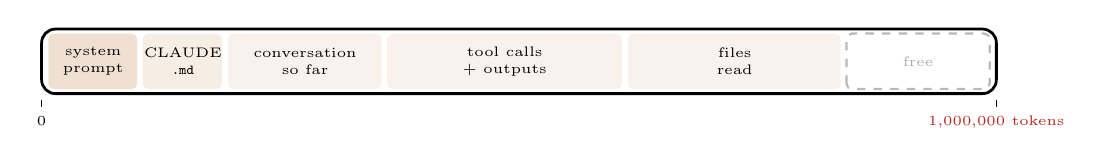
\begin{tikzpicture}[x=\linewidth, y=0.82cm]
  \draw[rounded corners=5pt, line width=1pt] (0,0) rectangle (1,1);
  \fill[brown!24, rounded corners=2pt] (0.007,0.07) rectangle (0.100,0.93);
  \node[align=center, font=\tiny] at (0.054,0.5) {system\\prompt};
  \fill[brown!14, rounded corners=2pt] (0.106,0.07) rectangle (0.189,0.93);
  \node[align=center, font=\tiny] at (0.148,0.5) {CLAUDE\\{\ttfamily.md}};
  \fill[brown!10, rounded corners=2pt] (0.195,0.07) rectangle (0.356,0.93);
  \node[align=center, font=\tiny] at (0.276,0.5) {conversation\\so far};
  \fill[brown!10, rounded corners=2pt] (0.362,0.07) rectangle (0.608,0.93);
  \node[align=center, font=\tiny] at (0.485,0.5) {tool calls\\+ outputs};
  \fill[brown!10, rounded corners=2pt] (0.614,0.07) rectangle (0.837,0.93);
  \node[align=center, font=\tiny] at (0.726,0.5) {files\\read};
  \draw[dashed, gray!55, rounded corners=2pt, line width=0.8pt] (0.843,0.07) rectangle (0.993,0.93);
  \node[font=\tiny, text=gray!65] at (0.918,0.5) {free};
  \draw[line width=0.6pt] (0,-0.20)--(0,-0.10);
  \draw[line width=0.6pt] (1,-0.20)--(1,-0.10);
  \node[anchor=north, font=\tiny] at (0,-0.20) {0};
  \node[anchor=north, font=\tiny, text=BrickRed] at (1,-0.20) {1,000,000 tokens};
\end{tikzpicture}

\column{0.38\textwidth}
\pause

% Cost-growth chart — width set to fill column after y-axis label overhead
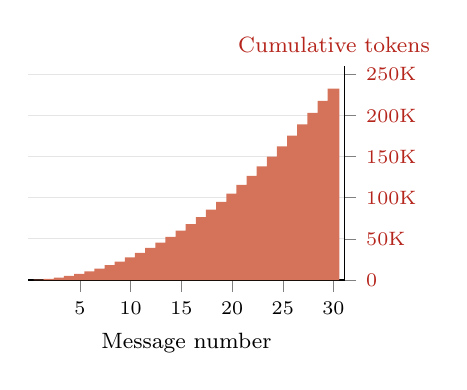
\begin{tikzpicture}

\begin{axis}[
    name=ax1,
    ybar, bar width=4.2pt,
    width=5.6cm, height=4.3cm,
    axis y line*=right,
    axis x line*=bottom,
    xlabel={Message number},
    xlabel style={font=\footnotesize},
    ylabel={Cumulative tokens},
    ylabel style={
        rotate=270,
        at={(1.3,1.1)},
        anchor=east,
        color=BrickRed,
        font=\footnotesize,
    },
    yticklabel style={color=BrickRed, font=\scriptsize},
    yticklabel pos=right,
    xticklabel style={font=\scriptsize},
    ymin=0, ymax=260000,
    xmin=0.5, xmax=30.5,
    xtick={5,10,15,20,25,30},
    ytick={0,50000,100000,150000,200000,250000},
    yticklabels={0,50K,100K,150K,200K,250K},
    scaled y ticks=false,
    ymajorgrids=true,
    grid style={gray!20, line width=0.4pt},
    tick align=outside,
    enlarge x limits=0.02,
]
\addplot[fill=BrickRed!55, draw=none] coordinates {
    (1,500)(2,1500)(3,3000)(4,5000)(5,7500)
    (6,10500)(7,14000)(8,18000)(9,22500)(10,27500)
    (11,33000)(12,39000)(13,45500)(14,52500)(15,60000)
    (16,68000)(17,76500)(18,85500)(19,95000)(20,105000)
    (21,115500)(22,126500)(23,138000)(24,150000)(25,162500)
    (26,175500)(27,189000)(28,203000)(29,217500)(30,232500)
};
\end{axis}
\end{tikzpicture}

\end{columns}

\end{frame}


%%%%%%%%%%%%%%
\begin{frame}
\frametitle{Getting the Most Out of Your Subscription}

\begin{itemize}
    \item Subscriptions have rolling limits --- fewer tokens per task means more use
    \vspace{.05in}
    \item How to use fewer tokens:
    	\begin{itemize}
            \item[$\circ$] Start a new session for each new task: context accumulates and raises costs
            \item[$\circ$] Store standing instructions once so you never repeat yourself
            \item[$\circ$] Be specific: vague prompts waste tokens and invite unfocused replies
            \item[$\circ$] Ask multiple things at once so less back and forth
             \item[$\circ$] Compact your chats/context window
        \end{itemize}	
    \vspace{.05in}
    \item Silly trick: start Claude when wake up so 5-hour window ends earlier in day
\end{itemize}

\end{frame}


\section{\textcolor{violet}{Claude Code / Codex Interfaces \vspace{0.3in}}}

%%%%%%%%%%%%%%
\begin{frame}
\frametitle{Three Ways to Use an Agentic Coding Tool}

\begin{itemize}
    \item \textbf{Terminal} (command line):
        \begin{itemize}
            \item[$\circ$] Most powerful; works directly in your project directory
            \item[$\circ$] Best for: running scripts, data analysis, replication tasks
        \end{itemize}
    \item \textbf{Desktop App}:
        \begin{itemize}
            \item[$\circ$] Friendlier interface; easier to get started
            \item[$\circ$] Projects feature: persistent context across sessions
            \item[$\circ$] Best for: drafting, quick questions, early exploration
        \end{itemize}
    \item \textbf{VS Code integration}:
        \begin{itemize}
            \item[$\circ$] Agent lives inside your editor --- see code and AI side by side
            \item[$\circ$] Best for: sustained development work, Git integration, Jupyter/Python
        \end{itemize}
\end{itemize}

\end{frame}




%%%%%%%%%%%%%%
\begin{frame}
\frametitle{Terminal vs.\ VS Code: Quick Comparison}

\begin{columns}[t]
\column{0.5\textwidth}
\textbf{Terminal (CLI)}
\vspace{.05in}
\begin{itemize}
    \item Lightweight; fast startup
    \item Works anywhere, incl.\ remote servers
    \item Keyboard-driven; fast for quick tasks
    \item No inline diffs; steeper setup
\end{itemize}

\column{0.5\textwidth}
\textbf{VS Code Extension}
\vspace{.05in}
\begin{itemize}
    \item Inline diffs; accept changes block-by-block
    \item Code \& AI panel side by side
    \item Best for large codebases, sustained work
    \item Heavier on CPU and memory
\end{itemize}
\end{columns}

\end{frame}


%%%%%%%%%%%%%%
\begin{frame}
\frametitle{Live Demo: Terminal}

\begin{itemize}
    \item \textcolor{gray}{\textit{$\triangleright$ Demo slide --- minimal text, walk through live}}
    \item Navigate to a project directory
    \item Ask Claude Code to describe what it sees
    \item Ask it to write a simple data task
\end{itemize}

\end{frame}




%%%%%%%%%%%%%%
\begin{frame}
\frametitle{Live Demo: Desktop App}

\begin{itemize}
    \item \textcolor{gray}{\textit{$\triangleright$ Demo slide --- minimal text, walk through live}}
    \item Create a Project and load context
    \item Same task as terminal --- compare experience
\end{itemize}

\end{frame}


%%%%%%%%%%%%%%
\begin{frame}
\frametitle{Live Demo: VS Code}

\begin{itemize}
    \item \textcolor{gray}{\textit{$\triangleright$ Demo slide --- walk through VS Code interface live}}
    \item Key panels: Explorer (files), Editor, Terminal, Source Control (Git), Extensions
    \item Claude Code panel: where you type prompts, see Claude's plan, approve edits
    \item Modes:
        \begin{itemize}
            \item[$\circ$] \textbf{Ask before edits}: Claude proposes each change; you approve
            \item[$\circ$] \textbf{Plan mode}: Claude writes a full plan in Markdown before doing anything
            \item[$\circ$] \textbf{Auto}: Claude acts autonomously (use carefully)
        \end{itemize}
\end{itemize}

\end{frame}


%%%%%%%%%%%%%%
\begin{frame}
\frametitle{Memory and Skills}

\begin{itemize}
    \item \textbf{CLAUDE.md} (memory): a file Claude reads at the start of every session
        \begin{itemize}
            \item[$\circ$] Store project context, preferences, and rules once --- never repeat yourself
            \item[$\circ$] Lives in your project folder; travels with the project
        \end{itemize}
    \vspace{.05in}
    \item \textbf{Skills} (\texttt{/command}): reusable slash commands for tasks you repeat
        \begin{itemize}
            \item[$\circ$] Stored as markdown files in \texttt{.claude/skills/}
            \item[$\circ$] Examples: \texttt{/summarize-paper}, \texttt{/make-table}, \texttt{/replicate}
        \end{itemize}
    \vspace{.05in}
    \item CLAUDE.md = always-on context \quad Skills = on-demand commands
\end{itemize}

\end{frame}

\section{\textcolor{violet}{Git: Version Control for Economists \vspace{0.3in}}}


%%%%%%%%%%%%%%
\begin{frame}
\frametitle{Why Git Matters for Research}

\begin{itemize}
    \item Version control = a complete history of every change to your code
    \item No more: \texttt{analysis\_v3\_FINAL\_revised2.do}
    \item Enables:
        \begin{itemize}
            \item[$\circ$] Rolling back to any prior version of your code
            \item[$\circ$] Working safely with coauthors and RAs without overwriting each other
            \item[$\circ$] Tracking exactly what changed between draft versions
            \item[$\circ$] Automatic replication audit trail
        \end{itemize}
    \vspace{.05in}
    \item The good news: Claude Code can handle all Git commands for you --- you just describe what you want
\end{itemize}

\end{frame}


%%%%%%%%%%%%%%
\begin{frame}
\frametitle{Key Git Concepts (No Commands Required)}

\begin{itemize}
    \item \textbf{Repository (repo)}: a folder whose history Git is tracking
    \item \textbf{Commit}: a snapshot of your code at a point in time, with a message
    \item \textbf{Push / Pull}: sync your local repo with GitHub (the remote copy)
    \item \textbf{Branch}: a parallel version of the code for a new feature or robustness check
    \item \textbf{Merge}: fold a branch back into the main code
    \vspace{.05in}
    \item Typical workflow for an economist:
        \begin{enumerate}
            \item Work on code; when something works, commit it
            \item Push to GitHub at end of day (backup + coauthor access)
            \item RA works on a branch; you review and merge
        \end{enumerate}
\end{itemize}

\end{frame}


%%%%%%%%%%%%%%
\begin{frame}
\frametitle{Git and Claude Code: What the Integration Looks Like}

\begin{itemize}
    \item \textcolor{gray}{\textit{$\triangleright$ Placeholder: screenshot or demo}}
    \item In VS Code: Git panel shows all changes; Claude Code can stage, commit, push on request
    \item You tell Claude: ``commit my changes with a descriptive message'' --- it writes the message too
    \item Branching for research: create a branch for each robustness check, merge if it works
    \item Connecting with Overleaf:
        \begin{itemize}
            \item[$\circ$] Overleaf Pro can sync with a GitHub repo
            \item[$\circ$] Alternatively: LaTeX Workshop extension in VS Code + local compilation
        \end{itemize}
\end{itemize}

\end{frame}


%%%%%%%%%%%%%%
\begin{frame}
\frametitle{Python in VS Code: Environments}

\begin{itemize}
    \item \textcolor{gray}{\textit{$\triangleright$ Demo slide --- Tanner}}
    \item Anaconda manages Python installations and packages
    \item Each project gets its own \textbf{environment}: a fixed set of packages and versions
        \begin{itemize}
            \item[$\circ$] Prevents conflicts between projects
            \item[$\circ$] Ensures others can reproduce your results exactly
        \end{itemize}
    \item Ask Claude Code to create and activate an environment for you
\end{itemize}

\end{frame}


%%%%%%%%%%%%%%
\begin{frame}
\frametitle{Running Python Code with Jupyter}

\begin{itemize}
    \item \textcolor{gray}{\textit{$\triangleright$ Demo slide --- Tanner}}
    \item Three modes in VS Code:
        \begin{itemize}
            \item[$\circ$] \textbf{Jupyter notebook} (\texttt{.ipynb}): interactive cells, inline output --- good for exploration
            \item[$\circ$] \textbf{Interactive window}: run \texttt{.py} scripts cell-by-cell --- best of both worlds
            \item[$\circ$] \textbf{Script} (\texttt{.py}): run the full pipeline --- best for production code
        \end{itemize}
    \item Claude Code can write, run, and debug Python in any of these modes
\end{itemize}

\end{frame}


\section{\textcolor{violet}{Setting Up Your Environment \vspace{0.3in}}}


%%%%%%%%%%%%%%
\begin{frame}
\frametitle{What You Need to Install}

\begin{itemize}
    \item Core tools (all free except AI subscription):
        \begin{enumerate}
            \item \textbf{VS Code} --- the editor (free)
            \item \textbf{Claude Code} --- VS Code extension + CLI (requires subscription)
            \item \textbf{Git} --- version control (free); create a GitHub account
            \item \textbf{Python} --- Anaconda distribution recommended (free)
        \end{enumerate}
    \item VS Code extensions to install:
        \begin{itemize}
            \item[$\circ$] Claude Code, GitLens, Jupyter, Python, Stata Enhanced (if applicable)
        \end{itemize}
    \item We have a step-by-step setup guide --- see handout / shared folder
\end{itemize}

\end{frame}


%%%%%%%%%%%%%%
\begin{frame}
\frametitle{Session 1 --- Key Takeaways}

\begin{enumerate}
    \item AI has perhaps most value added in coding
    \smallskip
    \item Agentic $\neq$ chatbot: reads files, writes and runs code, fixes errors, reports back
    \smallskip
    \item Two serious agentic options today: Claude Code and Codex
    \begin{itemize}
            \item[$\circ$] Pick one, learn it, reassess in 6 months
        \end{itemize}
    \item Tokens accumulate fast in long session --- start new session for each new task
    \smallskip
    \item Three interfaces (Terminal, Desktop, VS Code) and Git are your essential stack
\end{enumerate}

\end{frame}


%%%%%%%%%%%%%%
\begin{frame}
\frametitle{Questions?}

\begin{itemize}
    \item Questions on tools, concepts, or setup?
    \item Thoughts on how this fits your current workflow?
\end{itemize}

\end{frame}


\end{document}
